\section{Results}
\label{sec:Results}

This section documents the results of our many experiments designed to
characterize the performance of our data analysis workflows.  In
particular, we are interested in determining the additional overhead our
analysis places on the simulation and the efficiency with which it can be
done.  These data summarize evaluations run over the course of 9.36 million
core-hours of execution.  The results come from measurements taken from
instrumented code as well as the HPCToolkit profiling
tool~\cite{adhianto:hpctoolkit}.

\subsection{Experimental Setup}

All experiments were performed on the Cielo supercomputer housed at Los Alamos
National Laboratory.  Cielo is an 8,944-node Cray XE6 resource for the Advanced
Simulation and Computing (ASC) program and is jointly managed by Sandia National
Laboratories and Los Alamos National Laboratory under the New Mexico
Alliance for Computing at Extreme Scale (ACES) project.  Each node contains
two AMD Opteron 6136 (Magny-Cours) 8-way processor chips for a total of 16 cores
per node.  Each core has a peak computational speed of 2.4 GHz, leading to a total
theoretical peak of 1.37 Petaflops for the machine. The compute nodes each
have 32 GB of memory.  The interconnect consists of a proprietary Cray Gemini
Network with a 3D Torus topology and has a peak throughput rate of 6 GB/s/link.

This report includes strong scaling and weak scaling results from the
following CTH and analysis experiments.  These represent three different
workflows, two of which have two different configurations for a total of
five experiments.

\begin{description}

\item[\Insitu:] A CTH job that directly runs an \insitu analysis.  Thus,
  the \vda is performed in the same job and memory space as the
  simulation.  Within the \insitu workflow, we measure two variations of
  our watertight surface algorithm.

  \begin{description}

  \item[Baseline:] As described in Section~\ref{sec:UseCase}, the baseline
    version of the algorithm includes a somewhat unnecessary step of global
    communication to find AMR block neighbors.  We include results from
    this workflow for two reasons: First, we are not able to apply the same
    optimization to the \intransit and offline post-processing workflows,
    so this provides an apples-to-apples comparison of the benefit an
    \intransit approach could give using the same algorithm.  Second, we
    anticipate other important analysis algorithms could have similar
    communication characteristics.  For example, a connected components
    algorithm could require communication between most or all processes to
    resolve the connectivity of large fragments.

  \item[Refined:] As described in Section~\ref{sec:UseCase}, the refined
    version of the algorithm bypasses the step of global communication by
    retrieving the AMR block neighbors from the running CTH simulation.  We
    thus expect it to have better scaling performance.

  \end{description}

\item[\Intransit:] A CTH job that performs \intransit analysis using a
  separate allocation of compute nodes.  Data is transferred from the
  simulation to a service where \vda is performed asynchronously with
  respect to the simulation.  Within the \intransit workflow, we measure
  two job scheduling variations.

  \begin{description}

  \item[Extra nodes:] Allocate the CTH job with the same number of nodes as
    we would without the analysis, and then create a \vda service using
    extra nodes.  For example, if the simulation were normally to be run on
    256 nodes, then still schedule the simulation on 256 nodes and also
    schedule the \vda service on an additional 16 nodes.  This allocation
    represents a use case where there are additional compute nodes (perhaps
    with special OS, runtime, or hardware features) that could be used to
    perform analysis on behalf of the application.  For example, the
    suggested ``burst buffer'' architecture for the Trinity system may have
    special nodes with NVRAM and additional memory that would be
    appropriate for this type of \intransit analysis.

  \item[Internal nodes:] Divide the nodes normally allocated to the CTH job
    between the simulation and the \vda service.  For example, if the
    simulation were normally to be run on 256 nodes, then schedule the
    simulation on only 240 nodes and use the remaining 16 nodes to schedule
    the \vda service.  We use this workflow to find out if, given an equal
    number of resources for \insitu and \intransit, there might be
    situations where the preferable approach changes.
    
  \end{description}

\item [Spyplot file] A CTH job that writes Spyplot files instead of doing
  analysis.  At some point later a batch analysis job is run on the saved
  data.  This workflow represents the traditional post-processing approach.
  The number of nodes used matches the number used for analysis in the Extra
  nodes version of \intransit.

\end{description}

All applications complete 500 cycles (i.e., timestep calculations) of the
CTH code. The first four applications execute an analysis operation once
every 10 cycles.  For the Spyplot file application, we output spyplot data
at a fixed interval in simulated time, calculated so that the application
executed 51 I/O operations, equaling the number of analysis operations
performed by the \insitu and \intransit applications.  The number of nodes
used is the same as the \intransit application using external nodes. There is
no way to directly instruct CTH to output spyplot data every 10 cycles.  The
resulting data files are then loaded in a separate analysis job run at a latter
time.  This analysis was also performed on Cielo statically compiled from the
same code base as the \insitu code, but executed by ParaView's pvbatch
application.  The time to run the simulation, read and write files, and perform
the post-processing analysis are all summed together to get a processing time
for computation equivalent to that done in the \insitu and \intransit
workflows.

\begin{figure*}[p]
\begin{centering}
\vspace{-6pt}
\subfloat[\Insitu baseline.]{
  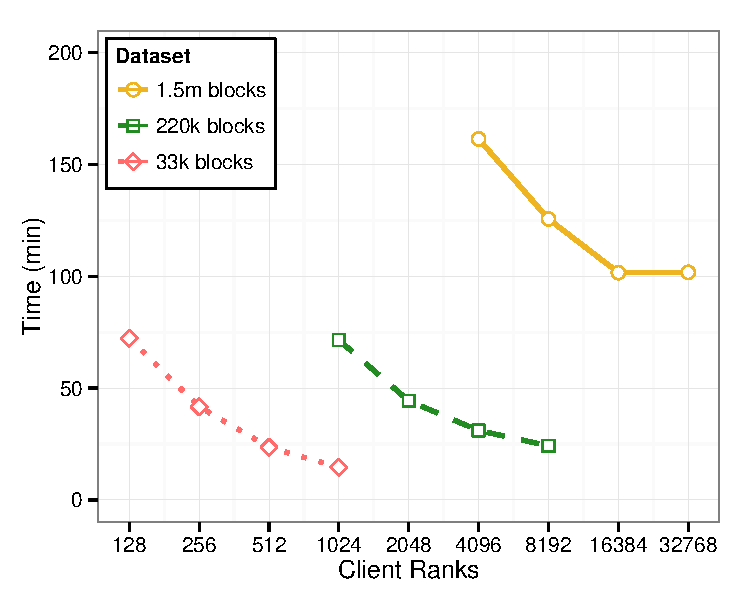
\includegraphics[width=0.48\linewidth]{figures/in-situ-unopt-line}
  \label{fig:in-situ-unopt-line}
}
\subfloat[\Insitu refined.]{
  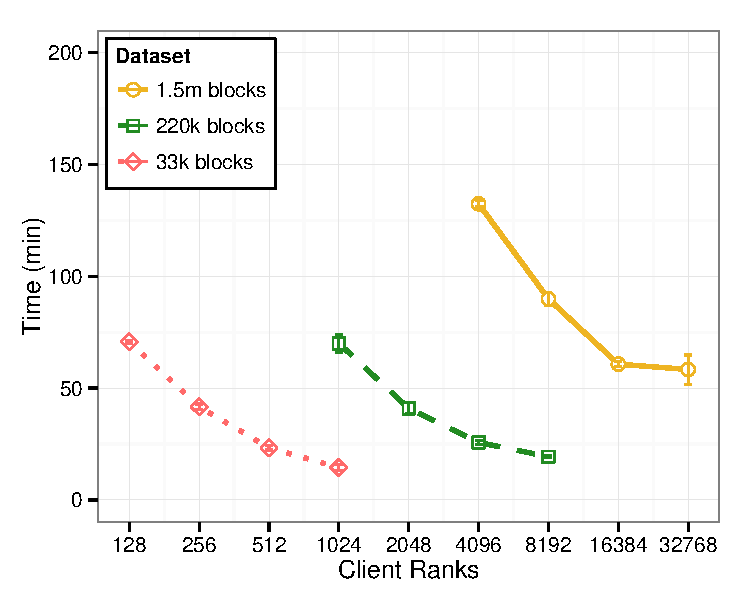
\includegraphics[width=0.48\linewidth]{figures/in-situ-opt-line}
  \label{fig:in-situ-opt-line}
}

\vspace{-6pt}
\subfloat[\Intransit with extra nodes.]{
  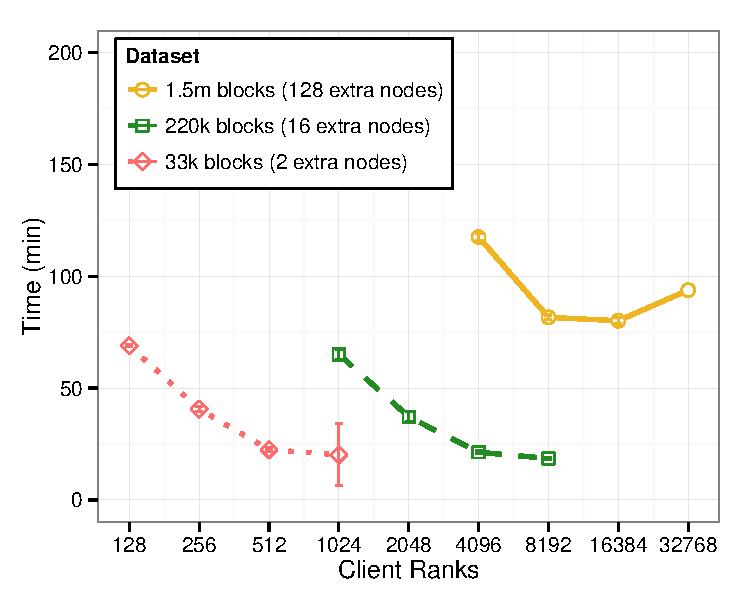
\includegraphics[width=0.48\linewidth]{figures/in-transit-extra-line}
  \label{fig:in-transit-extra-line}
}
\subfloat[\Intransit using internal nodes.]{
  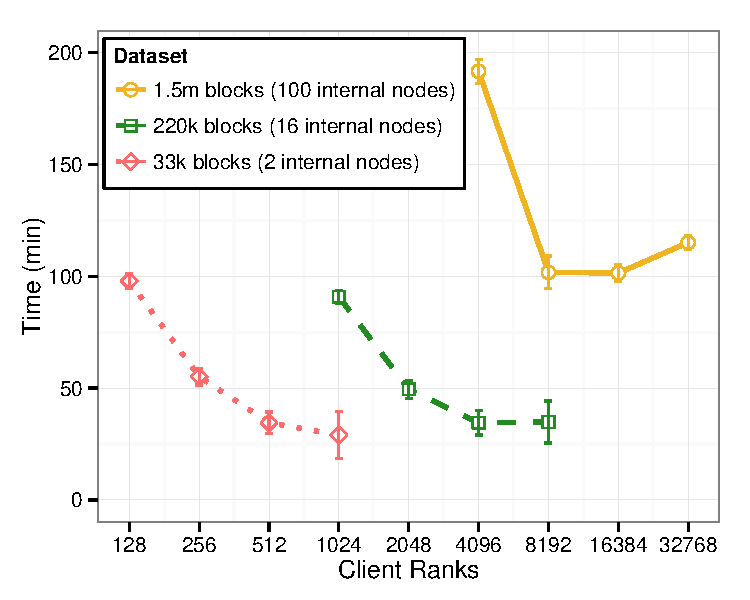
\includegraphics[width=0.45\linewidth]{figures/in-transit-inclusive-line}
  \label{fig:in-transit-inclusive-line}
}

\vspace{-6pt}
\subfloat[Spyplot I/O (post-processing analysis)]{
  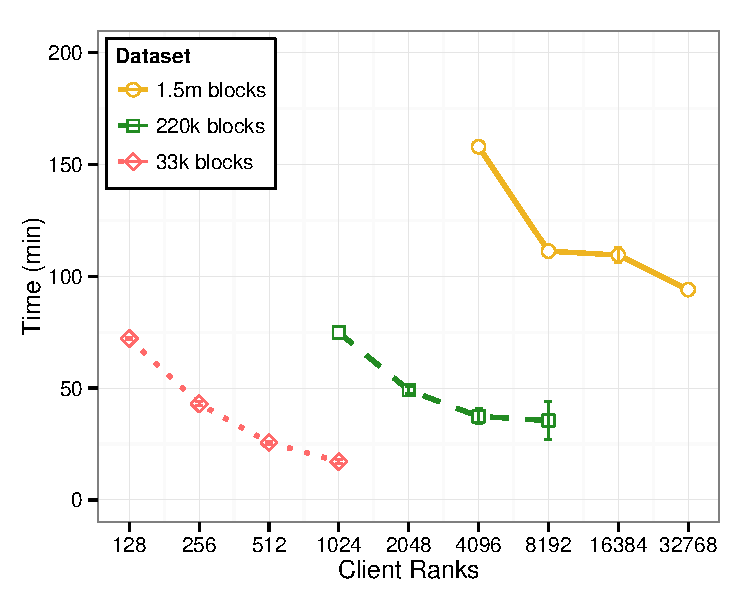
\includegraphics[width=0.48\linewidth]{figures/spyplot-file-line}
  \label{fig:spyplot-file-line}
}
\caption[Total runtime.]{Total runtime for 500-cycle runs of each
  workflow.}
\label{fig:runtime-individual}
\end{centering}
\end{figure*}


%%%%%%%%%%%%%%%%%%%%%% -- table ---
\begin{table}[htb]

\centering
\caption{Scaling Overview}
\label{tab:ScalingOverview}
\begin{tabular}{@{}lrrrrrrrr@{}}
\toprule
\qquad & \multicolumn{4}{c}{CTH}                                            & \multicolumn{4}{c@{}}{\Intransit Server} \\
       & \multicolumn{2}{c}{Most} & \multicolumn{2}{r}{\Intransit Internal} & \multicolumn{2}{r}{External Nodes} & \multicolumn{2}{r@{}}{Internal Nodes} \\
       & Cores & Nodes            & \qquad Cores & Nodes                     & \qquad Cores & Nodes                  & \quad Cores & Nodes \\
\midrule
\multicolumn{5}{@{}l@{}}{33K Blocks --- 5 levels} \\
& 128 & 8 & 96 & 6 & 16 & 2 & 16 & 2 \\
& 256 & 16 & 224 & 14 & 16 & 2 & 16 & 2 \\
& 512 & 32 & 480 & 30 & 16 & 2 & 16 & 2 \\
& 1,024 & 64 & 992 & 62 & 16 & 2 & 16 & 2 \\
\multicolumn{5}{@{}l@{}}{220K Blocks --- 6 levels} \\
& 1,024 & 64 & 768 & 48 & 128 & 16 & 128 & 16 \\
& 2,048 & 128 & 1,792 & 112 & 128 & 16 & 128 & 16 \\
& 4,096 & 256 & 3,840 & 240 & 128 & 16 & 128 & 16 \\
& 8,192 & 512 & 7,936 & 496 & 128 & 16 & 128 & 16 \\
\multicolumn{5}{@{}l@{}}{1.5M Blocks --- 7 levels} \\
& 4,096 & 256 & 2,496 & 156 & 1,024 & 128 & 800 & 100 \\
& 8,192 & 512 & 6,592 & 412 & 1,024 & 128 & 800 & 100 \\
& 16,384 & 1,024 & 14,784 & 924 & 1,024 & 128 & 800 & 100 \\
& 32,768 & 2,048 & 31,168 & 1,948 & 1,024 & 128 & 800 & 100 \\
& 65,536 & 4,096 & 63,936 & 3,996 & 1,024 & 128 & 800 & 100 \\
\bottomrule
\end{tabular}
\end{table}

%%%%%%%%%%%%%%%%%%%%%% -- table ---

For each application, we ran strong scaling experiments for three different
datasets.  Each data set comes from the same initial conditions but with a
different maximum level of refinement.  Thus, measurements of different job
sizes with different data set sizes provides a weak scaling overview.
Table~\ref{tab:ScalingOverview} shows the range of core sizes used for the
various experiments.  For every application we used the maximum 16
cores-per-node for the CTH client, since CTH is primarily bound by
computation and scales very well.  For the \intransit experiments in this
section, we used 8 cores for each service node.  The exception is in
Section~\ref{sec:node-scaling} where we discuss \intransit performance
under different core-per-node counts.

%The objective is run experiments with datasets representative of real
%production runs.  The minimum number of cores per dataset is limited by
%memory.  The maximum number of cores per dataset was decided to get scaling data,


\subsection{Total Execution Time}
\label{sec:TotalExecutionTime}

Our first consideration is the overall runtime of each workflow with each
data set and job size.

\begin{figure}[tbp]
\begin{centering}
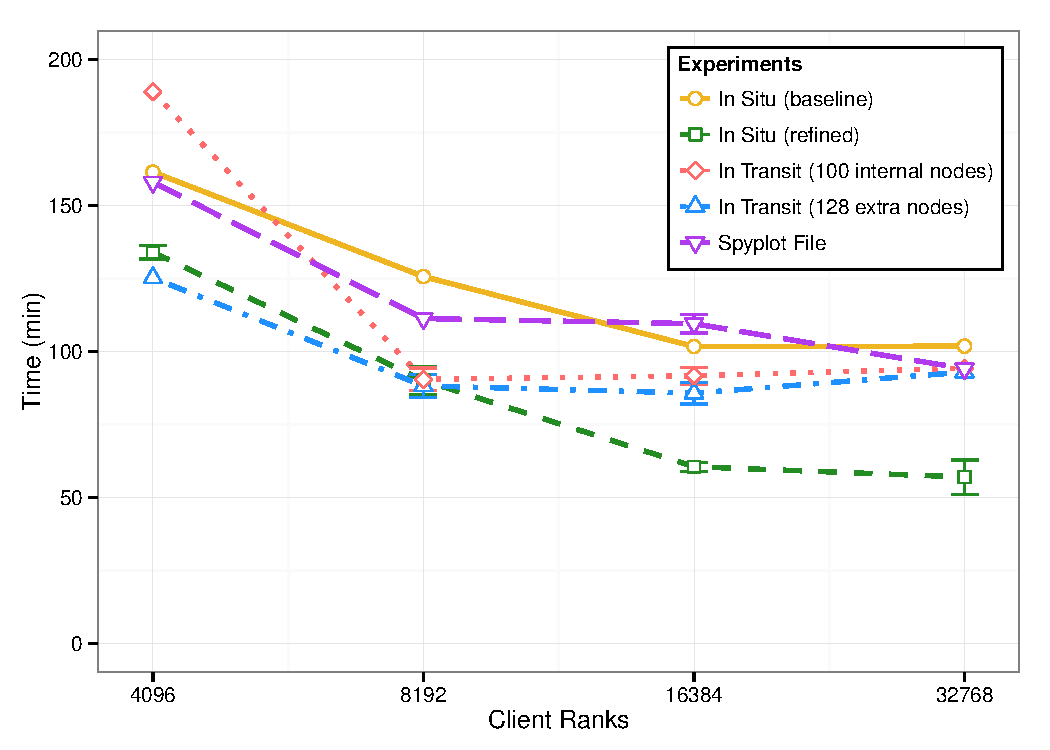
\includegraphics[scale=0.7]{figures/total-runtime-all}
\caption{Execution time comparison for the 1.5M block dataset.}
\label{fig:runtime-total}
\par\end{centering}
\end{figure}

Figures~\ref{fig:runtime-individual}~and~\ref{fig:runtime-total} show the
measured total execution time from each of the different workflows.  In cases
where we ran the same experiment multiple times, we plot the mean with error
bars representing the standard deviation from the mean. The set of plots in
Figure~\ref{fig:runtime-individual} show individual timings of each of the
workflows for each size dataset; the plot  in Figure~\ref{fig:runtime-total}
shows a direct comparison of all the  applications for the 1.5M block data set.
The results clearly show a ``sweet spot'' at 8K cores where the \intransit
approach, even though it is using a less scalable algorithm, performs the same
as the the refined version of \insitu.  At 16K and 32K, none of the codes
running analysis show significant improvement, the baseline \insitu and the
\intransit approaches actually take longer.  Perhaps the biggest reason is that
there is not enough work for the compute nodes.  At 32K cores, each core is
processing around 46 blocks/node, where the same size problem using 4K
nodes requires each core to process 366 blocks.  The key to making the
\intransit approach successful is being able to overlap computation and
analysis.  If the analysis portion does not scale particularly well, the
compute nodes need sufficient work to hide the analysis cost.

%% % Beacuse we have such large figures, the figures tend to be pushed way
%% % farther back in the document than they are referred to in the text, which
%% % is annoying when you are trying to read it.  This command will force all
%% % pending floats to be written out before continuing.  It can leave a large
%% % empty space in the text, but that ugliness is still better than the
%% % alternative.
%% \FloatBarrier

To better understand exactly where the time is being spent, we collect
detailed timings of each application using a combination of instrumented timers
and profiling tools (HPCToolkit).  Figure~\ref{fig:runtime-individual-bar} shows
the total runtime performance of the five workflows as a stacked bar plots
illustrating the portion of runtime associated with select functions.  For the
\insitu workflows, we measure the initialization and computational time of
CTH and the analysis/visualization.  For \intransit workflows, we measure
the initialization cost of CTH, the cost of transferring data to the service,
and the time the client waits for the server operation to complete. The wait
only occurs after CTH has finished its operation before the \vda is
complete.  If the \vda completes before CTH finishes its operation, then no
wait time occurs.

\begin{figure*}[htbp]
\begin{centering}
\vspace{-24pt}
\subfloat[\Insitu baseline.]{
  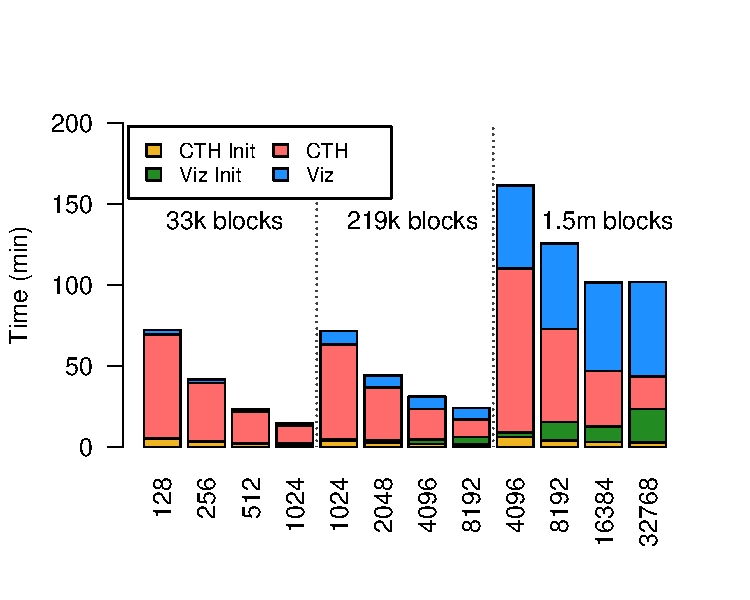
\includegraphics[width=0.48\linewidth]{figures/in-situ-unopt-bar}
  \label{fig:insitu-unopt-bar}
}
\subfloat[\Insitu refined.]{
  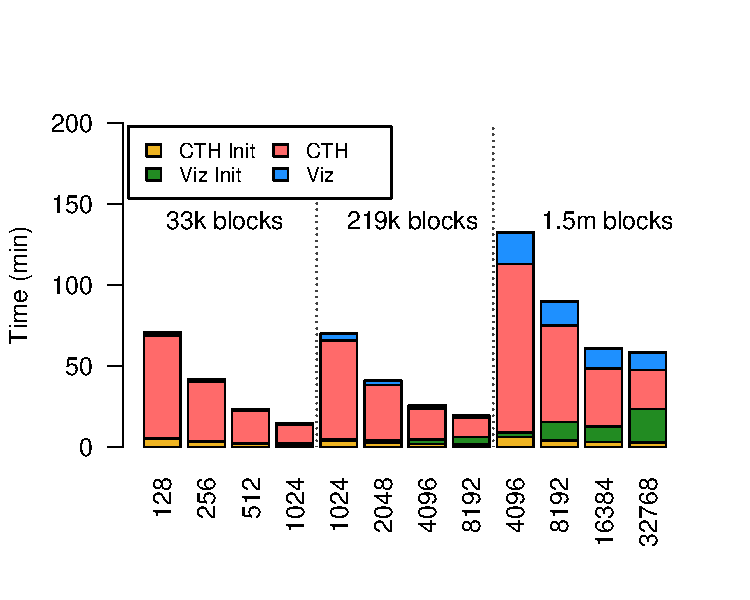
\includegraphics[width=0.48\linewidth]{figures/in-situ-opt-bar}
  \label{fig:insitu-opt-bar}
}

\vspace{-24pt}
\subfloat[\Intransit with extra nodes.]{
  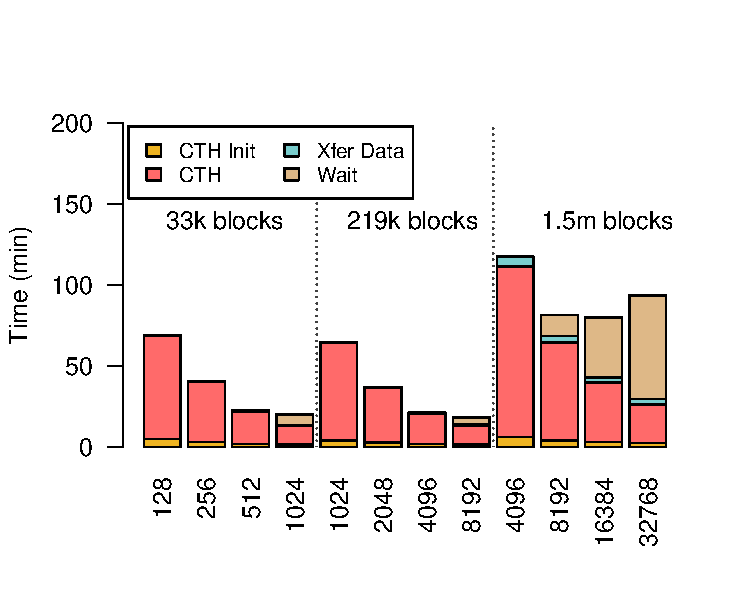
\includegraphics[width=0.48\linewidth]{figures/in-transit-extra-bar}
  \label{fig:intransit-extra-bar}
}
\subfloat[\Intransit using internal nodes.]{
  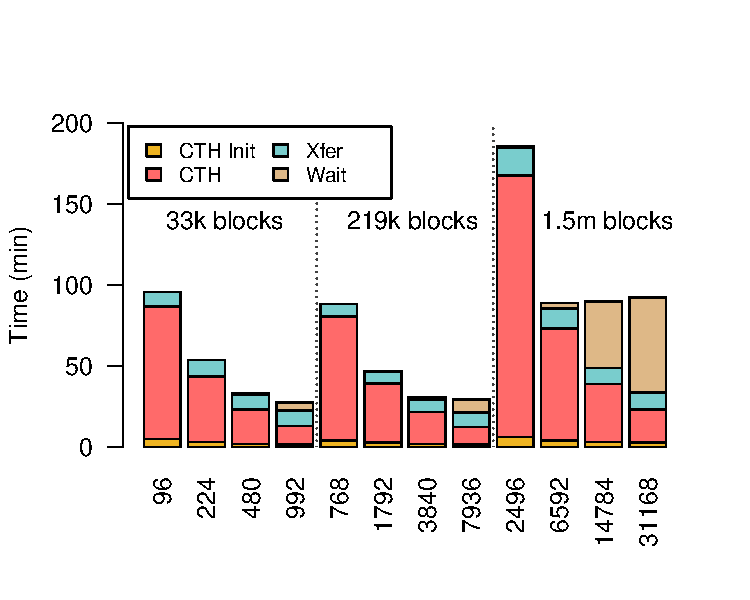
\includegraphics[width=0.48\linewidth]{figures/in-transit-inclusive-bar}
  \label{fig:intransit-inclusive-bar}
}

\vspace{-24pt}
\subfloat[Spyplot I/O (post-processing analysis)]{
  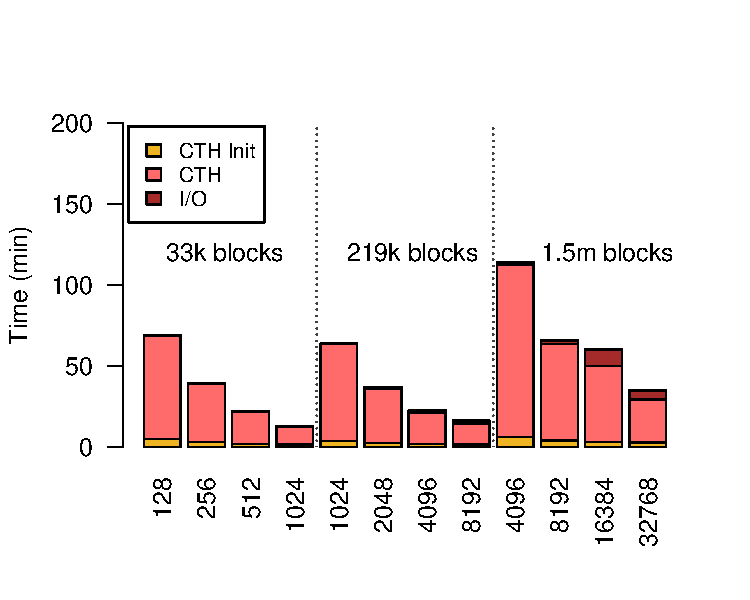
\includegraphics[width=0.5\linewidth]{figures/spyplot-file-bar}
  \label{fig:spyplot-file-bar}
}

\caption[Breakdown of operation timings.]{Illustration showing the
contributions of selected operations to the total execution times for each
application.}
\label{fig:runtime-individual-bar}
\end{centering}
\end{figure*}


Results from Figure~\ref{fig:insitu-unopt-bar} show that there is a clear
scaling problem with the analysis portion (labeled ``Viz'') of the baseline
\insitu workflow.  It almost appears as if the execution time is more
dependent on the problem size than the number of cores performing the analysis.
The refined version dramatically improves the performance.  This
corroborates our previous work\lcite{Fabian2012}, but we are now able to
take the scaling out to a larger scale to see that the performance appears
to be flattening out (although this might be in part due to a small number
of blocks per core).

Another important issue these timings reveal is that of the initialization
cost of the \vda.  Although the CTH initialization cost appears to decrease
as the core count increases, the initialization cost for analysis, ``Viz
Init,'' increases, accounting for more than 1/3 of the total time for a
500-cycle run.  For long runs, the initialization cost will get amortized,
but is still large enough to warrant further study.

The \intransit workflow results in
Figures~\ref{fig:intransit-extra-bar}~and~\ref{fig:intransit-inclusive-bar}
show that the \intransit approach effectively hides the analysis overhead
when the clients have sufficient compute resources.  For the 1.5M block
dataset, Figure~\ref{fig:intransit-extra-bar} shows that \intransit with an
extra 128 nodes successfully hides most of the cost of analysis at 4K and 8K
nodes, but the wait time at larger core counts eliminates any benefit of
\intransit using the baseline algorithm.

The \intransit workflow, shown in Figure~\ref{fig:intransit-inclusive-bar},
which carves out a subset of 100 nodes for analysis, has interesting
results as well.  Observe that the number of cores used for CTH is much
smaller, leading to an increase in the time spent doing CTH computation.
Even with this increase in computational cost, there is still benefit.  At
4K and 8K, all of the analysis cost is hidden.  At 8K, the total runtime is
slightly less than the refined version of \insitu.  This result is a bit
of a surprise given that they are both using the exact same number of
resources.

%The difference, it appears, is being able to hide the
%initialization as well as the analysis cost. \fix{Are we confident in
%  saying this? Perhaps describe what data leads to this conclusion.}  An
%improved algorithm for initialization could give the advantage back to the
%refined \insitu application.

An additional test of interest (not performed within the scope of this Milestone) would be to measure
performance of the \intransit workflows using the refined version of
the analysis algorithm.  If the the \intransit approach achieved the same
performance improvement shown by Figure~\ref{fig:insitu-opt-bar}, the
\intransit approach would be able to hide most of the analysis cost even at
large scale.  However, using the refined version of the analysis algorithm
would be different because the mesh decomposition changes when transferred
from client to server.  For the neighborhood information to remain
consistent, the I/O framework would have to report how data was
repartitioned so that the neighborhood information could be mapped to the
new decomposition.

Another surprising result is the performance of the spyplot file application.
For the size of datasets we studied, this application performed quite well, showing that
the Lustre file system on Cielo is quite strong.  The plots include the time
spent writing the spyplot files during the experiment and the measured time to
perform the analysis as a post-processing step.

\fix{Ron: more analysis.. get file sizes, data rates, ...}


% Beacuse we have such large figures, the figures tend to be pushed way
% farther back in the document than they are referred to in the text, which
% is annoying when you are trying to read it.  This command will force all
% pending floats to be written out before continuing.  It can leave a large
% empty space in the text, but that ugliness is still better than the
% alternative.
\FloatBarrier

\subsection{Time-Series Analysis}

To illustrate how operation performance changes throughout a single run
of the application, we selected one experiment and tracked the performance of
each 10-cycle period over a span of a 500 cycle run.  Since the ``Viz''
operation executes every 10 cycles, what is shown is the sum of 10-cycles worth
of CTH and the time spent by 1 analysis operation. We chose to evaluate
the experiments that use 8K processors of the 1.5M block dataset --- the ``sweet
spot'' mentioned in Section~\ref{sec:TotalExecutionTime} --- because it is one of
the interesting places where the performance of the refined \insitu application
and both \intransit applications all have similar total runtime.

\begin{figure}[tbp]
\begin{centering}
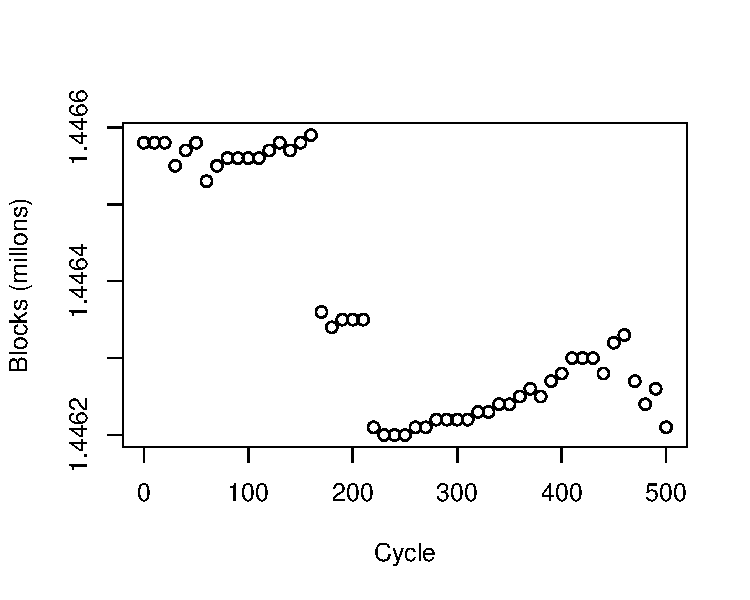
\includegraphics[scale=0.75]{figures/active-blocks-series}
\caption[Active Blocks]{Number of active blocks used in the course of a
500-cycle run of CTH.}
\label{fig:active-blocks}
\end{centering}
\end{figure}

Since we are running the adaptive-mesh refinement (AMR)
variant of CTH, the number of ``active'' blocks gets
recalculated by CTH at various points during a run. Since we expect this
to have an impact on CTH execution and \intransit transfer times, we first plot
the number of active blocks for our selected experiment in
Figure~\ref{fig:active-blocks}.  As simulation progresses, it is common for
the number of blocks to increase as finer resolution is needed to capture
cumulative physical effects.  This simulation has an interesting drop in
the number of blocks midway through; however, the drop in the number of
blocks is very slight (less than 0.01\%), so for practical purposes the
number of blocks is constant.

%In our particular execution, the number of
%active blocks actually decreases slightly (less than .01\%).

\begin{figure*}[bp]
\begin{centering}
\vspace{-24pt}
\subfloat[\Insitu baseline.]{
  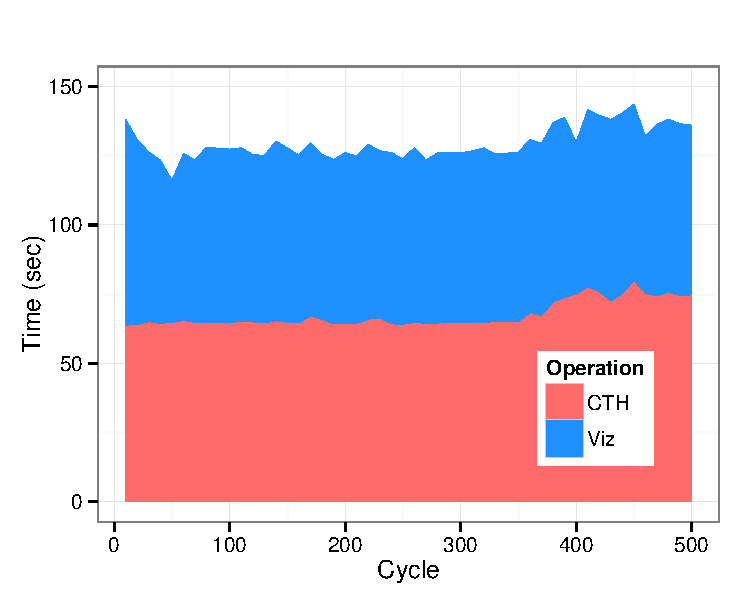
\includegraphics[width=0.48\linewidth]{figures/in-situ-unopt-series}
  \label{fig:insitu-unopt-series}
}
\subfloat[\Insitu refined.]{
  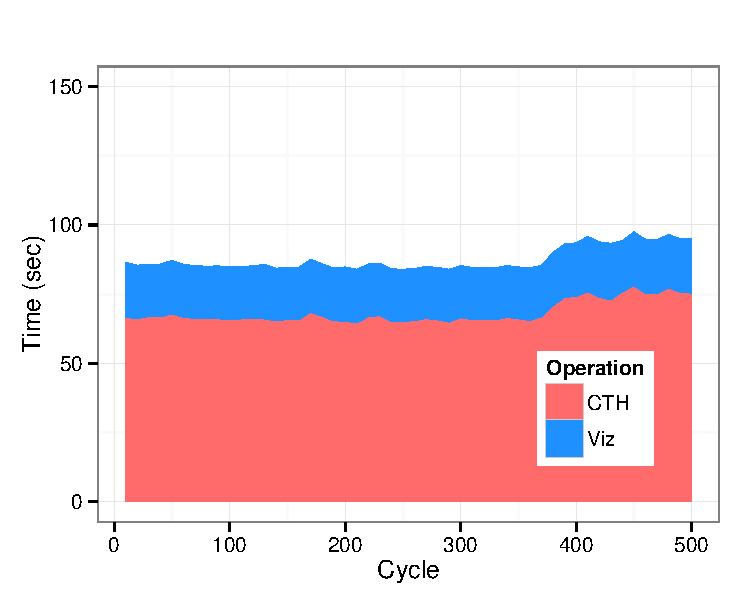
\includegraphics[width=0.48\linewidth]{figures/in-situ-opt-series}
  \label{fig:insitu-opt-series}
}

\vspace{-12pt}
\subfloat[\Intransit with extra nodes.]{
  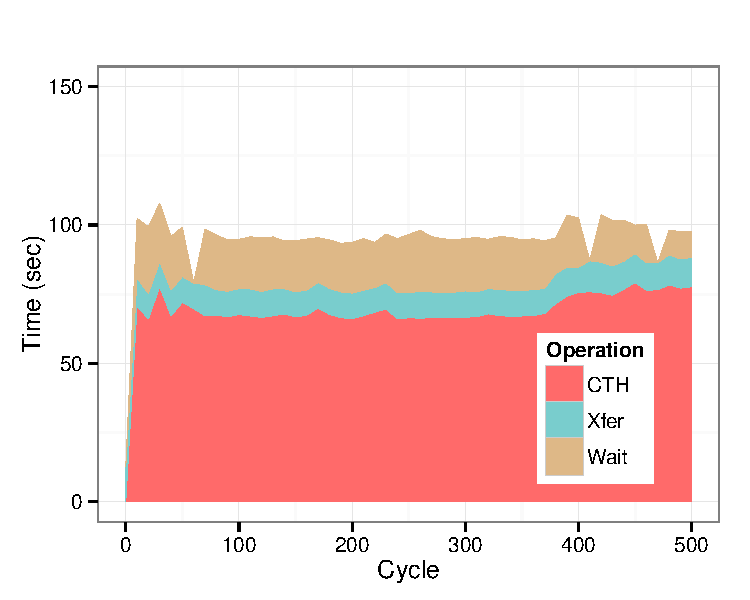
\includegraphics[width=0.48\linewidth]{figures/in-transit-extra-series}
  \label{fig:intransit-extra-series}
}
\subfloat[\Intransit using internal nodes.]{
  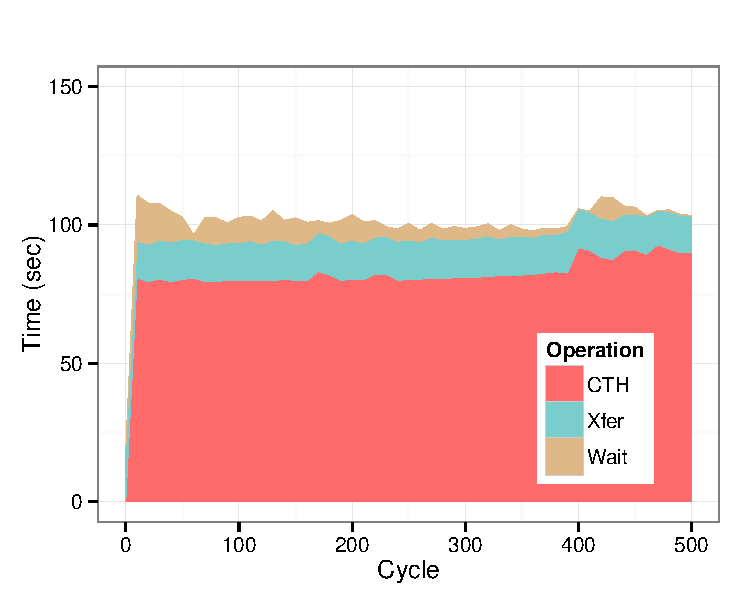
\includegraphics[width=0.48\linewidth]{figures/in-transit-inclusive-series}
  \label{fig:intransit-internal-series}
}


\caption[Time-series plots of experiments.]{Illustration showing the
contributions of selected operations for each 10-cycle period of a 500-cycle
CTH experiment.
}
\label{fig:time-series}
\end{centering}
\end{figure*}


Figure~\ref{fig:time-series} shows
the time contribution for a 10-cycle period of each important operation in the
\insitu and \intransit applications using 8K processors.  One observation
consistent across the different workflows is that the time spent performing
CTH computation tends to increase throughout the life of the application,
which is interesting considering that there not a significant increase in
either the number of blocks or the visualization processing time.

We also observe for the \intransit applications that as long as there is some
wait time, the total run time for each 10-cycle period remains relatively flat
throughout the life of the application.  We see this in both the \intransit
extra and \intransit inclusive experiments.  The reason for this is fairly
obvious.  If we assume the ``Viz'' operation on the service is essentially
constant, then the wait time should be the difference between the Viz time on
the service and the CTH time on the client.  As the CTH time increases, the
wait time decreases by the same amount.  Since the transfer time is close to
constant (it's based on the number of blocks), the total time at each 10-cycle
period remains about the same.


% Beacuse we have such large figures, the figures tend to be pushed way
% farther back in the document than they are referred to in the text, which
% is annoying when you are trying to read it.  This command will force all
% pending floats to be written out before continuing.  It can leave a large
% empty space in the text, but that ugliness is still better than the
% alternative.
\FloatBarrier

\subsection{Runtime Variance}

An increasingly important metric for HPC applications is runtime variance.  A
number of factors could contribute to inconsistent performance across multiple runs. Among
them are resource contention for memory, network, or storage systems, operating
system noise, and software techniques like garbage collection.
Instead of trying to understand the cause of inconsistent behavior in our
experiments, we to document the results with the intent of addressing
them further in future work.

\begin{figure*}[htbp]
\begin{centering}
%\vspace{-24pt}
\subfloat[CTH]{
  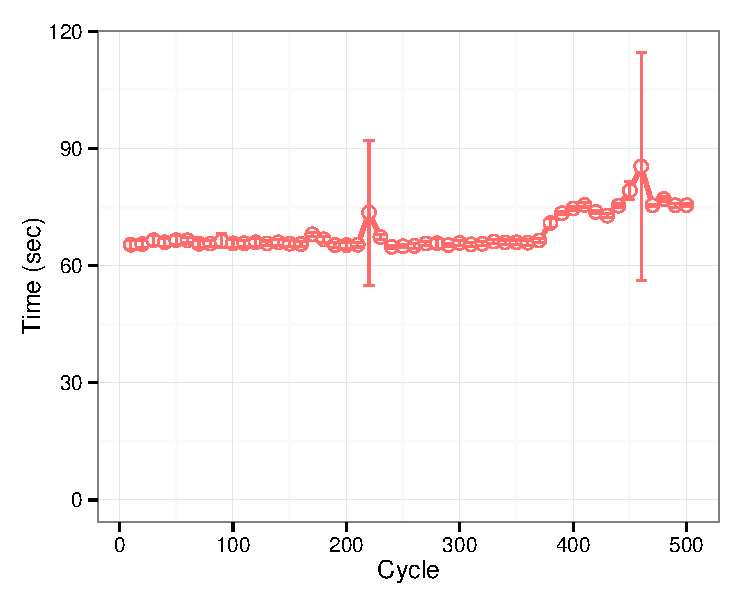
\includegraphics[width=0.48\linewidth]{figures/in-situ-opt-cth-variance}
  \label{fig:cth-variance}
}

\subfloat[\Insitu (baseline) analysis]{
  \includegraphics[width=0.48\linewidth]{figures/in-situ-unopt-viz-variance}
  \label{fig:insitu-unopt-variance}
}
\subfloat[\Insitu (refined) analysis]{
  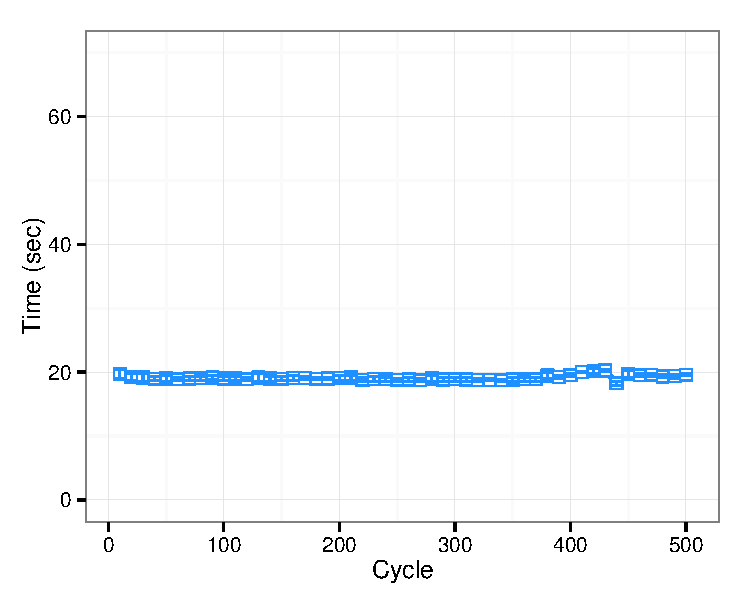
\includegraphics[width=0.48\linewidth]{figures/in-situ-opt-viz-variance}
  \label{fig:insitu-opt-variance}
}
\caption[Runtime variance of \insitu operations.]{Plots of the mean time and
standard error for CTH and the \insitu analysis operations.

\fix{Update baseline plots with latest data for final version.}
}
\label{fig:insitu-variance}
\end{centering}
\end{figure*}

\begin{figure*}[htbp]
\begin{centering}
%\vspace{-12pt}
\subfloat[\Intransit (extra nodes) transfer time.]{
  \includegraphics[width=0.48\linewidth]{figures/in-transit-extra-xfer-variance}
  \label{fig:intransit-extra-xfer-variance}
}
\subfloat[\Intransit (extra nodes) wait time.]{
  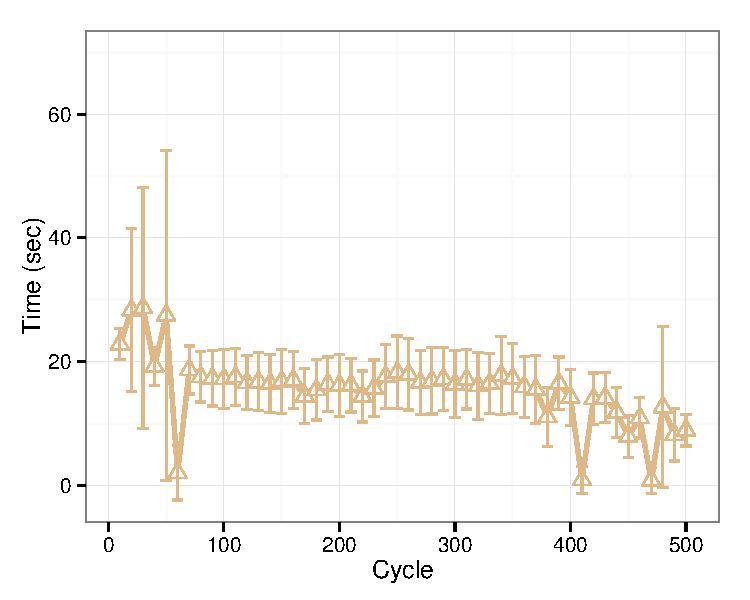
\includegraphics[width=0.48\linewidth]{figures/in-transit-extra-wait-variance}
  \label{fig:intransit-extra-wait-variance}
}

\subfloat[\Intransit (inclusive) transfer time.]{
  \includegraphics[width=0.48\linewidth]{figures/in-transit-inclusive-xfer-variance}
  \label{fig:intransit-inclusive-xfer-variance}
}
\subfloat[\Intransit (inclusive) wait time.]{
  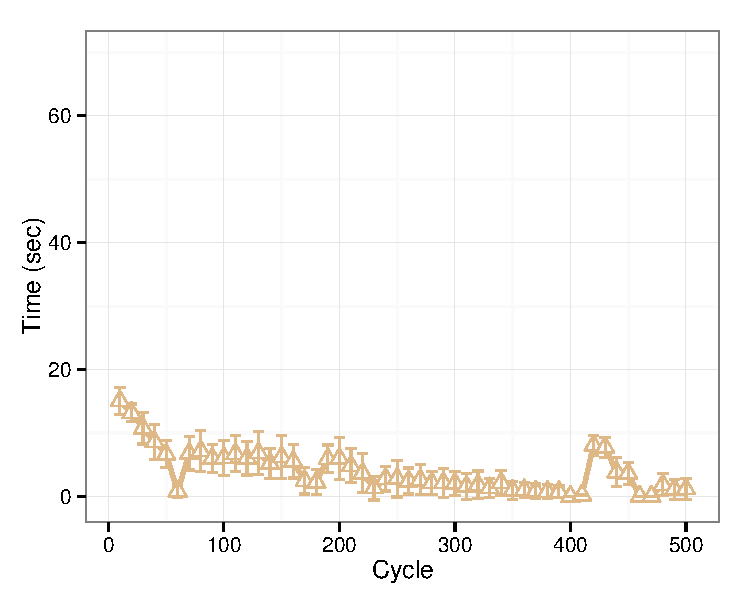
\includegraphics[width=0.48\linewidth]{figures/in-transit-inclusive-wait-variance}
  \label{fig:intransit-inclusive-wait-variance}
}

\caption[Runtime variance of \intransit operations.]{Plots of the mean time and
standard error for the \intransit transfer and wait operations.

\fix{Update inclusive plots with latest data for final version.} }
\label{fig:intransit-variance}
\end{centering}
\end{figure*}


The plots in Figures \ref{fig:insitu-variance} and
\ref{fig:intransit-variance} show the mean and standard error (the standard
deviation from the mean) of the important \insitu and \intransit operations
for the 8k-core experiments.  In each plot, we gathered data from five or
more 500-cycle experiments.  Most of our measurements show a small amount
of variance between experiments.  There are some outlier measurements in
Figures \ref{fig:cth-variance} and \ref{fig:intransit-extra-wait-variance}
that we attribute to another event running concurrently on Cielo by
happenstance causing contention.  The transfer time of \intransit workflows
(Figures \ref{fig:intransit-extra-xfer-variance} and
\ref{fig:intransit-inclusive-xfer-variance}) have more variance than the
rest, which we attribute to the Cielo job scheduler not taking into account
the communication between the client and server jobs.


% Beacuse we have such large figures, the figures tend to be pushed way
% farther back in the document than they are referred to in the text, which
% is annoying when you are trying to read it.  This command will force all
% pending floats to be written out before continuing.  It can leave a large
% empty space in the text, but that ugliness is still better than the
% alternative.
\FloatBarrier


\subsection{Scaling Analysis}
\label{sec:node-scaling}

\subsubsection{Block Processing Rate}

One way to get a good understanding of the scalability of an operation is
to look at the throughput or processing rate.  In this case, we look at the
rate at which the analysis operation processes blocks as we increase the
number of client cores.

\fix{Ron, in talking to Nathan, it seems that the
  blocks/second rate shouldl take into account all of the blocks, not just
  the active blocks.  This is because the analysis has to run on inactive
  blocks because they are frequently part of the main mass.  However, I
  suspect these measurements are using ``active blocks'' instead of actual
  blocks.}



\begin{figure*}[htbp]
\begin{centering}
\vspace{-12pt}
\subfloat[\Insitu baseline.]{
  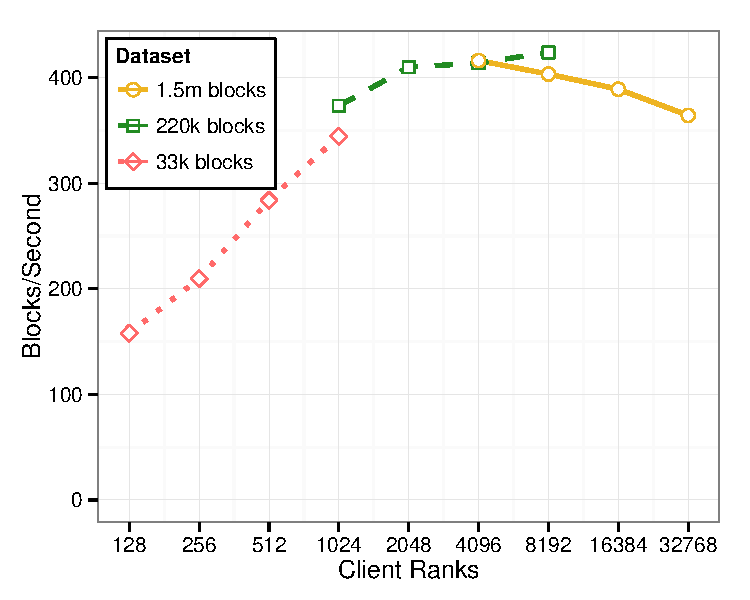
\includegraphics[width=0.45\linewidth]{figures/in-situ-unopt-rate}
  \label{fig:in-situ-unopt-rate}
}
\subfloat[\Insitu refined.]{
  \includegraphics[width=0.45\linewidth]{figures/in-situ-opt-rate}
  \label{fig:in-situ-opt-rate}
}

\subfloat[\Intransit with extra nodes.]{
  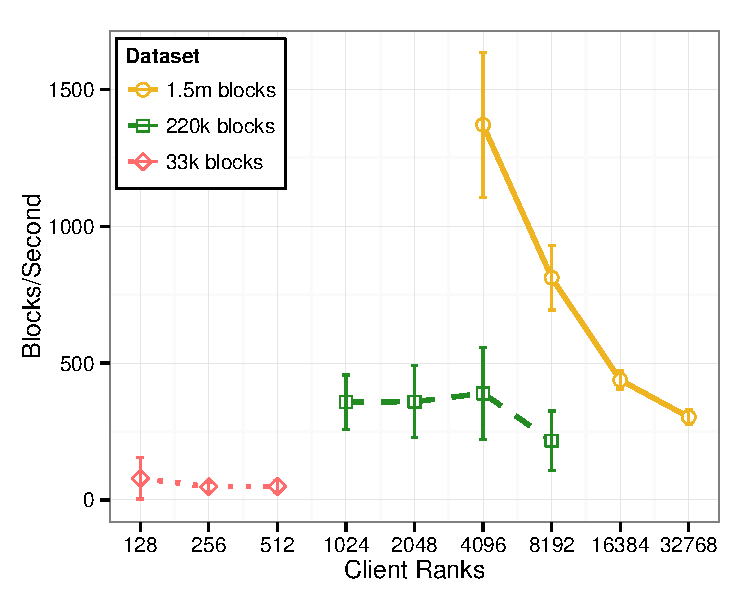
\includegraphics[width=0.45\linewidth]{figures/in-transit-extra-rate}
  \label{fig:in-transit-extra-rate}
}
\subfloat[\Intransit with internal nodes.]{
  \includegraphics[width=0.45\linewidth]{figures/in-transit-inclusive-rate}
  \label{fig:in-transit-inclusive-rate}
}


\caption[Processing rate of analysis.]{Processing rate of analysis portions of
the four different applications.}
\label{fig:processing-rates}
\end{centering}
\end{figure*}

Figure~\ref{fig:processing-rates} shows the processing rates of the
analysis portion of the \intransit applications and the ``effective''
processing rate of the analysis portion (transfer time plus wait time) of
the \intransit applications.  Note that the effective \intransit rate does
not include any processing time overlapped with the simulation execution,
and thus could be much larger than the actual processing rate.  As we
expect, the baseline application scales fine for the small data set, but
starts to really drop off for the medium and large data.  We see a dramatic
improvement in the \insitu refined application as it scales consistently
well all the way to 32K cores.  The \intransit applications are also not
that surprising.  Since we use a fixed number of nodes for a dataset, we
expect the effective processing rate to be essentially flat.  The dropoff
for the medium and large datasets is due to the excessive waiting,
identified in Figures \ref{fig:intransit-extra-bar} and
\ref{fig:intransit-inclusive-bar}.



\subsubsection{Node scaling for \intransit experiments}

In this section, we evaluate performance of the \intransit applications when
using different numbers of cores/node for the \intransit service.  To better
understand the impact of changing the core count for the services, consider the
three HPCToolkit-generated performance traces in
Figure~\ref{fig:node-scaling-traces}.  The traces show a 10-cycle window
of execution for a 128-core job using 1 server node. For this small experiment,
we used a dataset of only 5k blocks.

\begin{figure*}[htbp]
\begin{centering}
\vspace{-12pt}
\subfloat[\Intransit with 2 cores/server.]{
  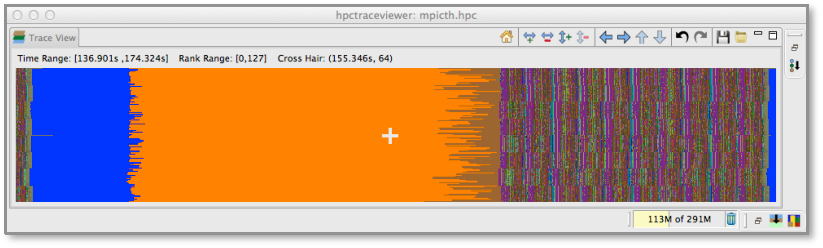
\includegraphics[width=0.95\linewidth]{figures/service-2-cores}
  \label{fig:service-2-cores}
}

\subfloat[\Intransit with 4 cores/server.]{
  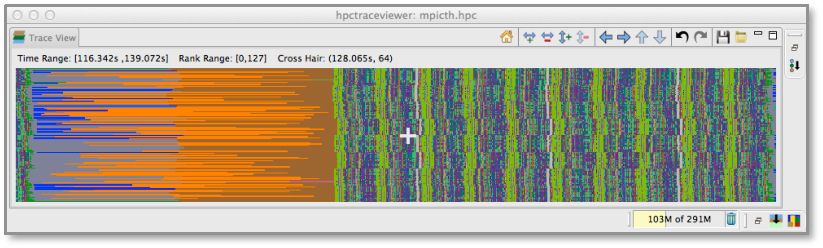
\includegraphics[width=0.95\linewidth]{figures/service-4-cores}
  \label{fig:service-4-cores}
}

\subfloat[\Intransit with 8 cores/server.]{
  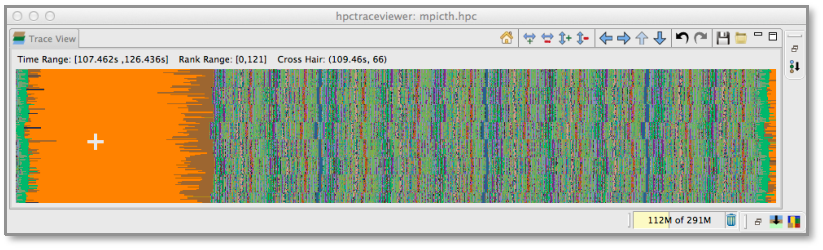
\includegraphics[width=0.95\linewidth]{figures/service-8-cores}
  \label{fig:service-8-cores}
}


\caption[Performance trace of 128-core run with different core
counts.]{HPCToolkit-generated traces showing a 10-cycle window of execution
for a 128-core job using 2, 4, and 8 cores for the server nodes.}
\label{fig:node-scaling-traces}
\end{centering}
\end{figure*}

The tracing results show a dramatic difference in network performance and wait
time between all three of the experiments.  We believe the relatively poor
network performance in the 2-core experiment is caused by contention. Because
only 2 cores can process the bulk-data requests at a time, the clients are
either waiting for network transfers to complete, or the are waiting for the
server to finish copying the data to a server buffer, causing the request to
sit in the server's pending queue. The larger wait time on the 2-core experiment
tells us that for this size  problem, there is a computational benefit to
increasing the number of cores  performing the analysis.



\begin{figure*}[htbp]
\begin{centering}
\vspace{-12pt}
\subfloat[Total time (33k blocks).]{
  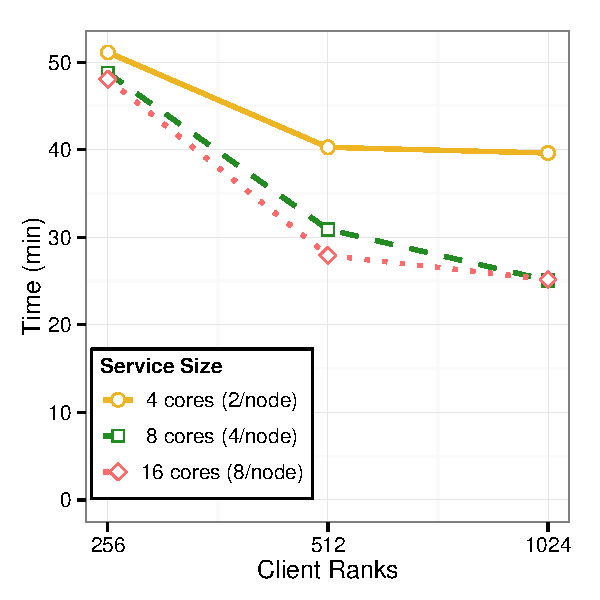
\includegraphics[width=0.3\linewidth]{figures/in-transit-33k-total}
  \label{fig:in-transit-33k-total}
}
\subfloat[Transfer time (33k blocks).]{
  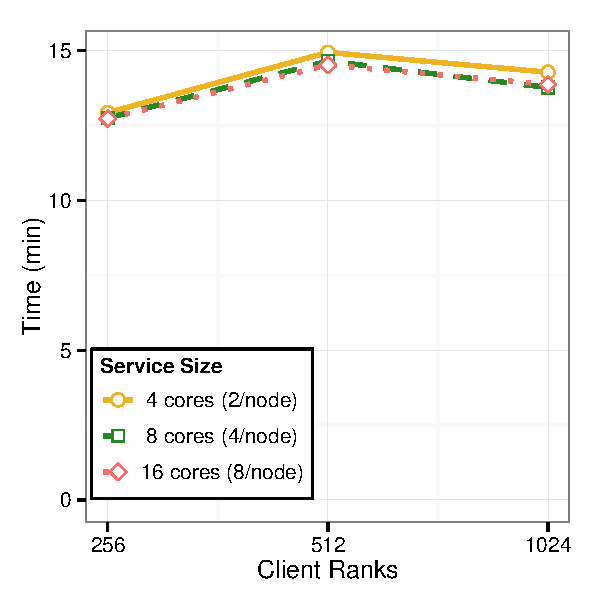
\includegraphics[width=0.3\linewidth]{figures/in-transit-33k-xfer}
  \label{fig:in-transit-33k-xfer}
}
\subfloat[Wait time (33k blocks).]{
  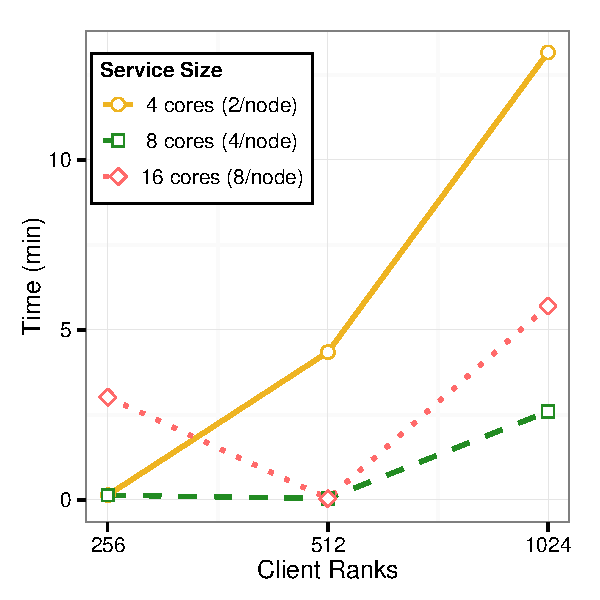
\includegraphics[width=0.3\linewidth]{figures/in-transit-33k-wait}
  \label{fig:in-transit-33k-wait}
}

\subfloat[Total time (218k blocks).]{
  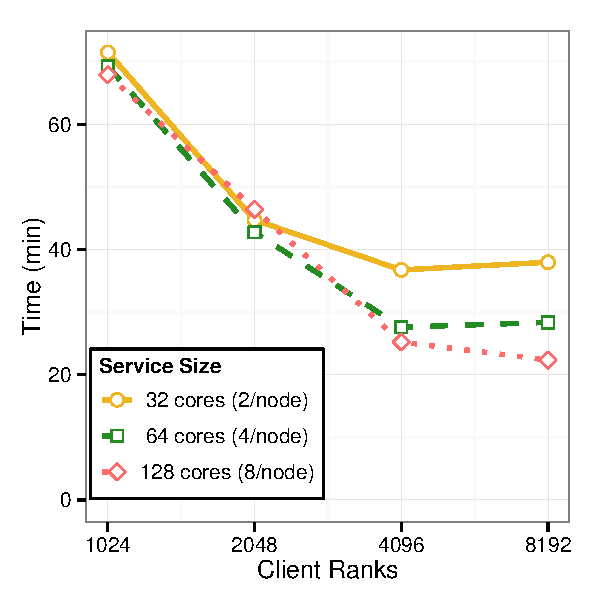
\includegraphics[width=0.3\linewidth]{figures/in-transit-218k-total}
  \label{fig:in-transit-218k-total}
}
\subfloat[Transfer time (218k blocks).]{
  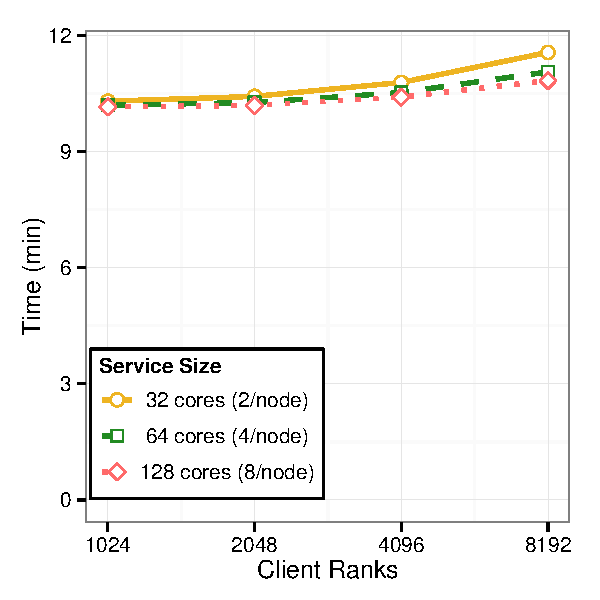
\includegraphics[width=0.3\linewidth]{figures/in-transit-218k-xfer}
  \label{fig:in-transit-218k-xfer}
}
\subfloat[Wait time (218k blocks).]{
  \includegraphics[width=0.3\linewidth]{figures/in-transit-218k-wait}
  \label{fig:in-transit-218k-wait}
}

\subfloat[Total time  (1.5m blocks).]{
  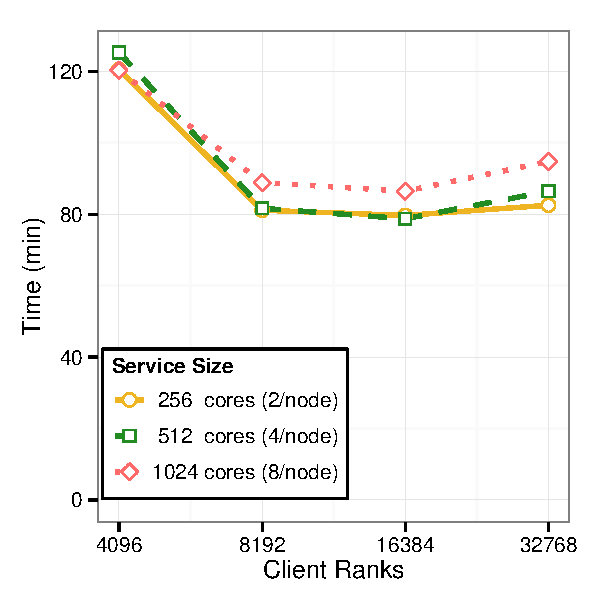
\includegraphics[width=0.3\linewidth]{figures/in-transit-1m-total}
  \label{fig:in-transit-1m-total}
}
\subfloat[Transfer time (1.5m blocks).]{
  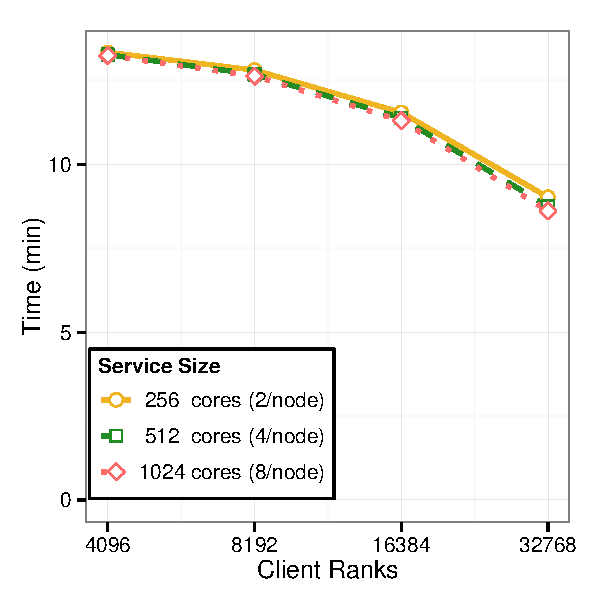
\includegraphics[width=0.3\linewidth]{figures/in-transit-1m-xfer}
  \label{fig:in-transit-1m-xfer}
}
\subfloat[Wait time (1.5m blocks).]{
  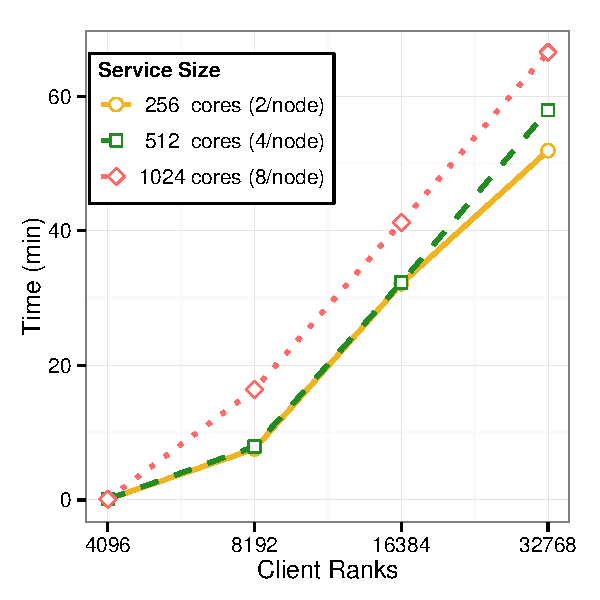
\includegraphics[width=0.3\linewidth]{figures/in-transit-1m-wait}
  \label{fig:in-transit-1m-wait}
}

\caption[\Intransit core scaling.] {\Intransit
performance for 2, 4, and 8 cores per server node.}
\label{fig:core-scaling}
\end{centering}
\end{figure*}

The plots in Figure~\ref{fig:core-scaling} show differences in the total,
transfer, and wait times for the 2, 4, and 8 cores/node runs of the \intransit
(extra) application for the three different data sets.  \fix{need more time to
digest and understand these plots.  May need to run more results.}


%%%%%%%%%%%%%%%%%%%%%%%%%%%%%%%%%%%%%%


% Beacuse we have such large figures, the figures tend to be pushed way
% farther back in the document than they are referred to in the text, which
% is annoying when you are trying to read it.  This command will force all
% pending floats to be written out before continuing.  It can leave a large
% empty space in the text, but that ugliness is still better than the
% alternative.
\FloatBarrier

\subsection{Memory}
The following memory plots were taken by examining free memory on the nodes
using /proc/meminfo.  Measuring free memory is conservative because it also
accounts for caches and buffers, so although you may run out of free memory in
a system, the execution will not immediately fail due to memory freed from
those other sources.  However, these are an indication of the worst case
possible.  On Cielo there are 16 cores per node and in each case the nodes were
 loaded with 16 MPI ranks executing the statically linked executable.

In order to understand CTH memory usage results, it is important to note that
CTH preallocates memory based on a value for ``max number of blocks'' provided
through the input deck.  Because of this, CTH memory usage is highly impacted
by the user specification.  In this case we ran the results with what we
believe are reasonable values for ``max number of blocks'' given the size of the
problem.  Figure~\ref{fig:MaxBlocks} shows the corresponding max blocks for
each run.

\begin{figure}[htb]
  \centering
  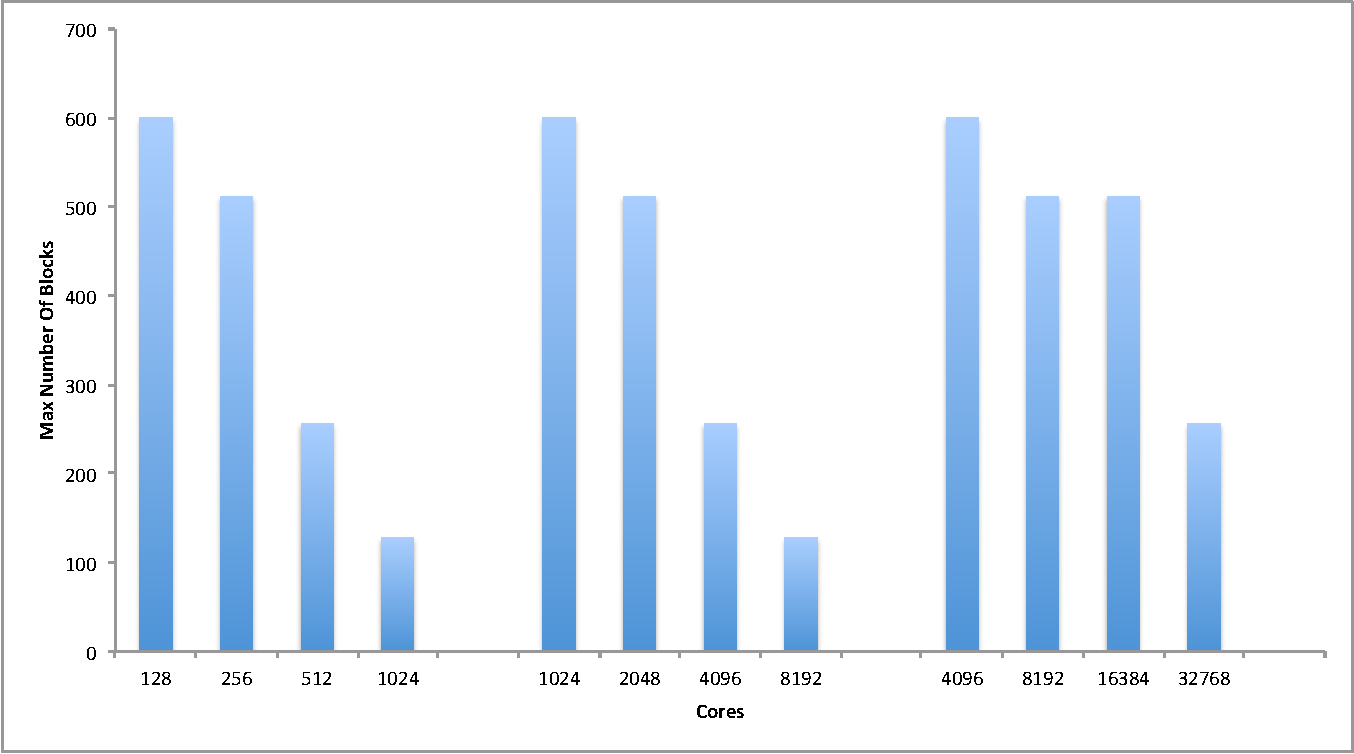
\includegraphics[width=\linewidth]{figures/MaxNumberOfBlocks}
  \caption[Max number of blocks parameter.]{A plot of the ``max number of
    blocks'' parameter supplied to CTH for each run.}
  \label{fig:MaxBlocks}
\end{figure}

Figure~\ref{fig:MemoryUsageAll} provides an overview of all memory
measurements taken for the system.  The memory taken by CTH is quite flat,
as expected, for each run.  However, even though the size of the mesh
changes throughout the simulation, the memory overhead for \insitu and
\intransit runs changes only moderately.  Thus, for the rest of the results
analysis, we summarize all measurements as simply the maximum value, which
is a reasonable representation of all values.

\begin{figure}[htb]
  \centering
  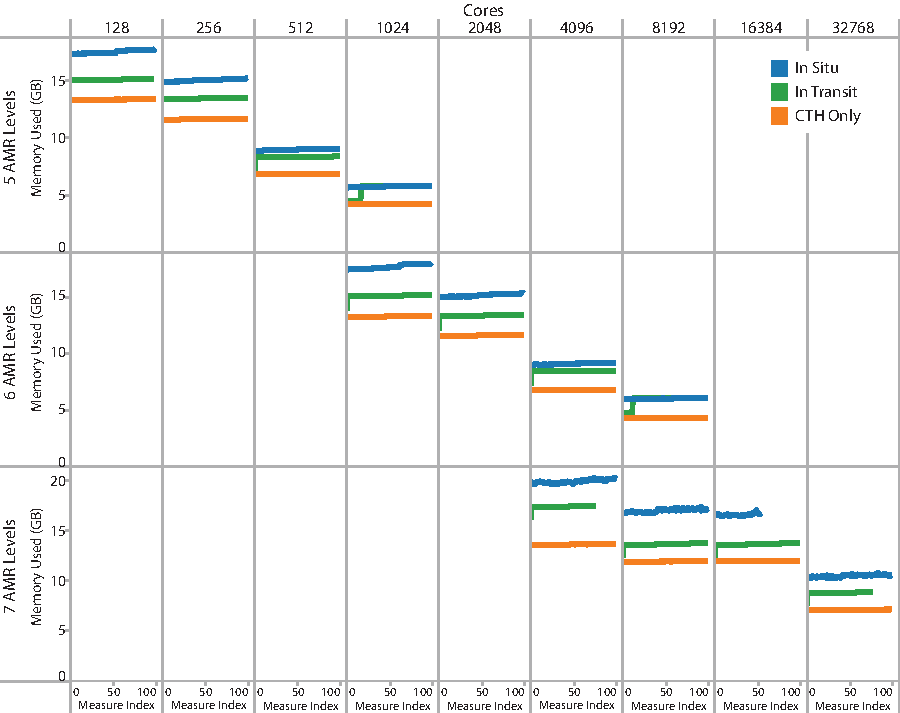
\includegraphics[width=\linewidth]{figures/MemoryUsageAll}
  \caption[Memory usage plot matrix.]{Matrix of all measurements taken for
    memory usage comparisons.  Each measurement is the total memory in use
    in a node (so for \insitu and \intransit memory includes both CTH
    simulation and overhead).  Each measurement is plotted as the maximum
    memory use in all nodes at the time the measurement was taken.}
  \label{fig:MemoryUsageAll}
\end{figure}

Figure~\ref{fig:MemoryInSituPerNode} gives a summary of the extra memory
used when using Catalyst for \insitu analysis during our experiments.
Likewise, Figure~\ref{fig:MemoryInTransitPerNode} gives the same summary
for the \intransit memory overhead for the nodes within the simulation
(memory usage on the separate analysis job is not given).  In all cases the
added overhead is less than 50\% than the memory used by CTH itself, and in
most cases the additional overhead is significantly smaller than that.

\begin{figure}[htb]
  \centering
  \includegraphics[width=\linewidth]{figures/MemoryUsageInSituPerNode}
  \caption{Plot of average per node memory usage of the \insitu run on Cielo.}
  \label{fig:MemoryInSituPerNode}
\end{figure}

\begin{figure}[htb]
  \centering
  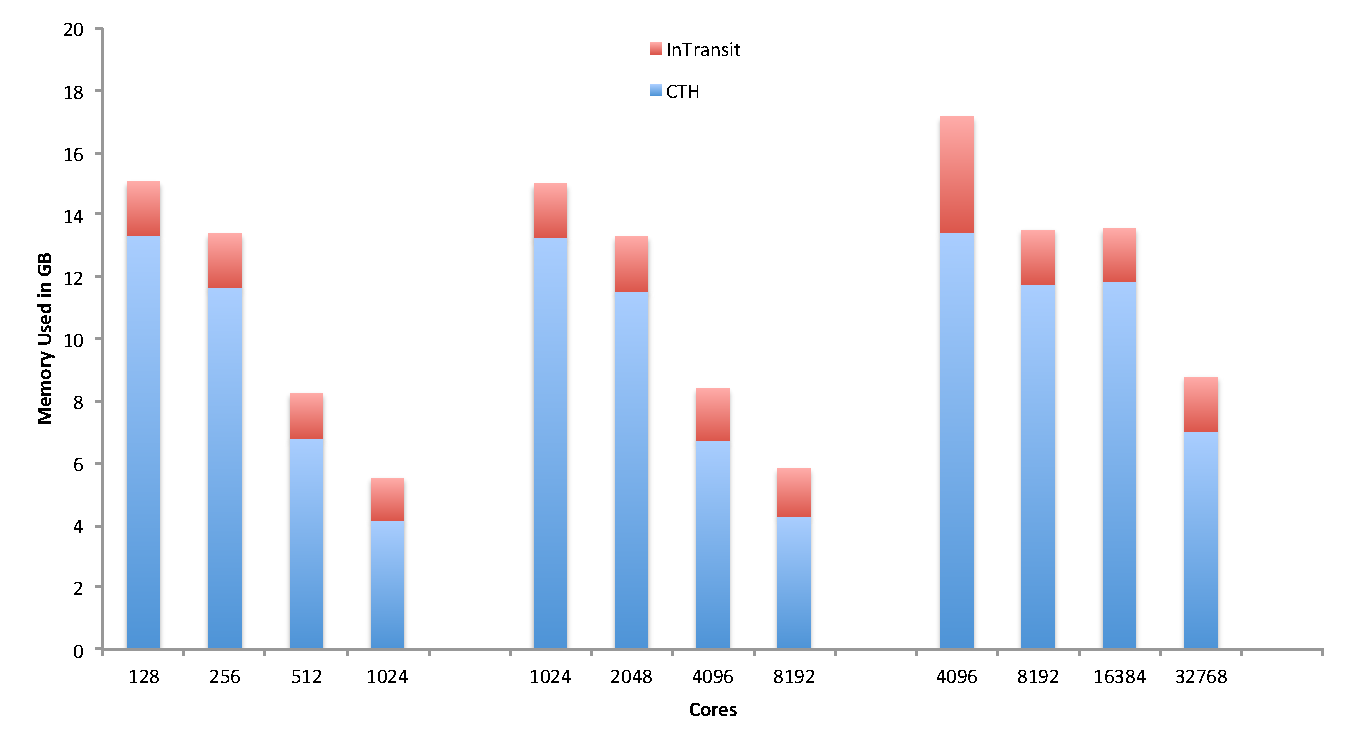
\includegraphics[width=\linewidth]{figures/MemoryUsageInTransitPerNode}
  \caption{Plot of average per node memory usage of the \intransit run on Cielo.}
  \label{fig:MemoryInTransitPerNode}
\end{figure}

Figure~\ref{fig:MemoryCompare} compares the amount of memory per node added
when using \insitu versus \intransit.  As expected, the \intransit approach
requires a smaller memory overhead than \insitu within the nodes of the
simulation.  Thus, \intransit could be a better option when the simulation
requires as much memory per process as possible, but the \intransit
approach also requires separate nodes to be reserved for the analysis,
which also may cause the total amount of available simulation memory to be
reduced if nodes must be taken away from the simulation.

\begin{figure}[htb]
  \centering
  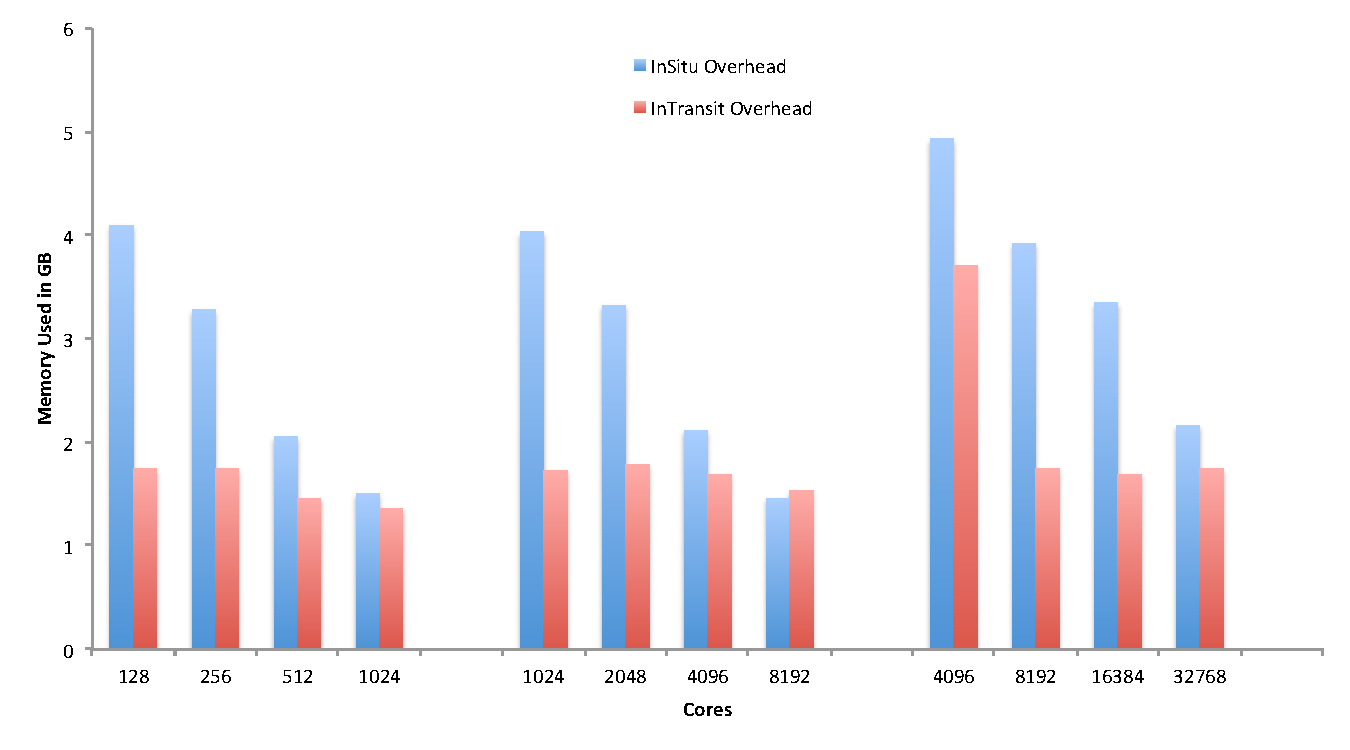
\includegraphics[width=\linewidth]{figures/MemoryUsageCompare}
  \caption{Plot of the average overhead per node of both \insitu and \intransit}
  \label{fig:MemoryCompare}
\end{figure}


